\begin{name}
	{\tenchude}
	{\tendethi}
	{THPT Kim Liên - Hà Nội}
	{\thoigian}
\end{name}

\Opensolutionfile{ans}[ans/2-TT-KimLien-HaNoi-L1-NH21-22]
%câu 1
\begin{ex}%[dự án 16 tex đề thi thử Sở-Đinh Bích Hảo]%[2D1B5-3]
\immini{Cho hàm số bậc bốn  $y=f(x)$  có đồ thị là đường cong trong hình.
Số nghiệm thực của phương trình  $2f(x)+3=0$  là
\choice
{\True $4$}
{$1$}
{$3$}
{$2$}}{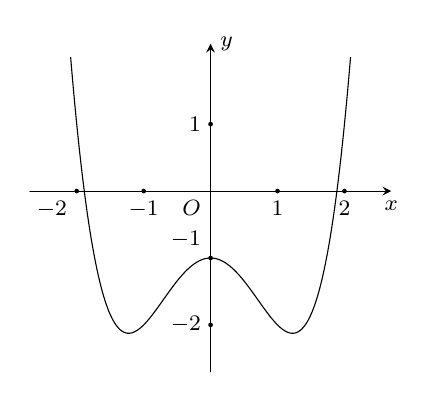
\begin{tikzpicture}[scale=0.85, font=\footnotesize, line join=round, line cap=round, >=stealth]
\def\xmin{-2.5}\def\xmax{2.5}\def\ymin{-2.5}\def\ymax{2}
\draw[->] (\xmin-0.2,0)--(\xmax+0.2,0) node[below] {\footnotesize $x$};
\draw[->] (0,\ymin-0.2)--(0,\ymax+0.2) node[right] {\footnotesize $y$};
\draw (0,0) node [below left] {\footnotesize $O$};
\draw (-2,0) node [below left] {\footnotesize $-2$};
\foreach \x in {-1,1,2}\fill (\x,0) circle(1pt) node [below] {\footnotesize $\x$};
\foreach \y in {-2,1}\fill (0,\y) circle(1pt) node [left] {\footnotesize $\y$};
\fill (-2,0) circle (1pt);
\fill (0,-1) circle (1pt) node[above left]{\footnotesize $-1$};
\clip (\xmin,\ymin) rectangle (\xmax,\ymax);
\draw[smooth,samples=200,domain=\xmin:\xmax] plot (\x,{1/2*((\x)^4)+-3/2*((\x)^2)+-1});
\end{tikzpicture}}
\loigiai{
\immini{Ta có $2f(x)+3=0 \Leftrightarrow f(x)=-\dfrac{3}{2}$.\\
Đường thẳng $y=-\dfrac{3}{2}$ cắt đồ thị hàm số đã cho tại bốn điểm phân biệt nên phương trình $2f(x)+3=0$ có bốn nghiệm phân biệt.}
{
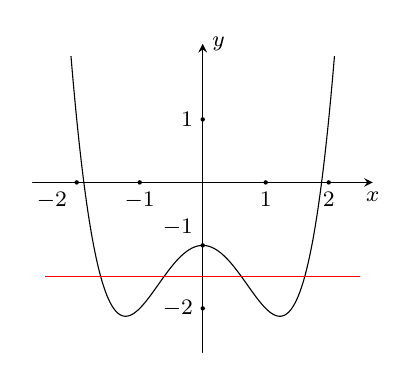
\begin{tikzpicture}[scale=0.8, font=\footnotesize, line join=round, line cap=round, >=stealth]
\def\xmin{-2.5}\def\xmax{2.5}\def\ymin{-2.5}\def\ymax{2}
\draw[->] (\xmin-0.2,0)--(\xmax+0.2,0) node[below] {\footnotesize $x$};
\draw[->] (0,\ymin-0.2)--(0,\ymax+0.2) node[right] {\footnotesize $y$};
\draw (-2,0) node [below left] {\footnotesize $-2$};
\foreach \x in {-1,1,2}\fill (\x,0) circle(1pt) node [below] {\footnotesize $\x$};
\fill (-2,0) circle (1pt);
\foreach \y in {-2,1}\fill (0,\y) circle(1pt) node [left] {\footnotesize $\y$};
\fill (0,-1) circle (1pt) node[above left]{\footnotesize $-1$};
\clip (\xmin,\ymin) rectangle (\xmax,\ymax);
\draw[smooth,samples=200,domain=\xmin:\xmax] plot (\x,{1/2*((\x)^4)+-3/2*((\x)^2)+-1});
\draw[red,smooth,samples=200,domain=\xmin:\xmax] plot (\x,{-3/2});
\end{tikzpicture}   
}}
\end{ex}

%câu 2
\begin{ex}%[dự án 16 tex đề thi thử Sở-Đinh Bích Hảo]%[2D3Y2-1]
	Cho hàm số $y=f(x)$  có  đạo hàm trên đoạn $[1;2]$, $f(1)=1$ và $f(2)=2$. Tính \break $I=\displaystyle \int \limits_1^2 f'(x)\mathrm{d}x$.
\choice
{ $I=3$}
{\True $I=1$}
{$I=-1$}
{$I=\dfrac{7}{2}$}
\loigiai{
Ta có $I=\displaystyle \int \limits_1^2 f'(x)\mathrm{d}x=f(x) \Big|_1^2=f(2)-f(1)=2-1=1$.}
\end{ex}

%câu 3
\begin{ex}%[dự án 16 tex đề thi thử Sở-Đinh Bích Hảo]%[2D3B2-1]
Biết  $F(x)=x^4$ là một nguyên hàm của hàm số  $f(x)$ trên  $\mathbb{R}$. Giá trị của    $I=\displaystyle \int \limits_{-1}^2 [6x+f(x)]\mathrm{d}x$ bằng
\choice
{ $\dfrac{78}{5}$}
{\True $24$}
{$33$}
{$I=\dfrac{123}{5}$}
\loigiai{
Ta có $I=\displaystyle \int \limits_{-1}^2 [6x+f(x)]\mathrm{d}x=\left(3x^2+x^4\right)\Big|_{-1}^2=24.$}
\end{ex}

%câu 4
\begin{ex}%[dự án 16 tex đề thi thử Sở-Đinh Bích Hảo]%[2H3Y3-2]
Trong không gian  $Oxyz$, cho đường thẳng  $d$  đi qua điểm  $M(1;-4;3)$  và có một véc-tơ chỉ phương là  $\vec{u}=(5;4;-2)$. Phương trình của  đường thẳng  $d$ là
\choice
{ $\heva{&x=5+t\\&y=4-4t\\&z=-2+3t}$}
{\True $\heva{&x=1+5t\\&y=-4+4t\\&z=3-2t}$}
{$\heva{&x=1-5t\\&y=4-4t\\&z=3-2t}$}
{$\heva{&x=1-5t\\&y=-4-4t\\&z=3-2t}$}
\loigiai{
Phương trình đường thẳng   $d$ là $\heva{&x=1+5t\\&y=-4+4t\\&z=3-2t.}$}
\end{ex}

%câu 5
\begin{ex}%[dự án 16 tex đề thi thử Sở-Đinh Bích Hảo]%[1D3B3-2]
Cho cấp số cộng $(u_n)$ có $u_1=2$, $u_1+u_2=5$. Tìm công sai $d$ của cấp số cộng trên.
\choice
{ $d=2$}
{\True $d=1$}
{$d=3$}
{$d=\dfrac{3}{2}$}
\loigiai{
Ta có $u_1+u_2=5 \Leftrightarrow u_1+u_1+d=5 \Leftrightarrow 2u_1+d=5 \Leftrightarrow d=5-2u_1=1$.}
\end{ex}

%câu 6
\begin{ex}%[dự án 16 tex đề thi thử Sở-Đinh Bích Hảo]%[2D1Y4-1] 
Tiệm cận đứng của đồ thị hàm số  $y=\dfrac{2x+3}{x-2}$  là đường thẳng có phương trình
\choice
{ $y=-2$}
{\True $x=2$}
{$x=-2$}
{$y=2$}
\loigiai{
Tập xác định $\mathscr{D}=\mathbb{R} \setminus \{2\}$.\\
Ta có $\lim \limits_{x \to 2^+}\dfrac{2x+3}{x-2}=+\infty$.\\
Vậy đường tiệm cận đứng của đồ thị hàm số  $y=\dfrac{2x+3}{x-2}$  là đường thẳng  $x=2$.}
\end{ex}

%câu 7
\begin{ex}%[dự án 16 tex đề thi thử Sở-Đinh Bích Hảo]%[2D4Y1-1]
Xác định phần ảo của số phức   $z=18-12i$.
\choice
{ $12i$}
{ $12$}
{\True $-12$}
{$-12i$}
\loigiai{
Phần ảo của số phức   $z=18-12i$ là $-12$.}
\end{ex}

%câu 8
\begin{ex}%[dự án 16 tex đề thi thử Sở-Đinh Bích Hảo]%[2H2Y2-1]
Thể tích $V$  của khối cầu có bán kính $R$  được tính theo công thức nào dưới đây?
\choice
{ $V=\dfrac{1}{3}\pi R^3$}
{ $V=4\pi R^3$}
{\True $V=\dfrac{4}{3}\pi R^3$}
{$V=\pi R^3$}
\loigiai{
Công thức tính thể tích của khối cầu có bán kính  $R$  là  $V=\dfrac{4}{3}\pi R^3$.}
\end{ex}

%câu 9
\begin{ex}%[dự án 16 tex đề thi thử Sở-Đinh Bích Hảo]%[2D1B1-1]
Cho hàm số  $y=\dfrac{5x+9}{x-1}$. Khẳng định nào sau đây là đúng?
\choice
{ Hàm số nghịch biến trên $(-\infty;1)\cup (1;+\infty)$}
{ Hàm số đồng biến trên $(-\infty;1)\cup (1;+\infty)$}
{\True Hàm số nghịch biến trên $(-\infty;1)$ và $(2;+\infty)$}
{Hàm số nghịch biến trên $\mathbb{R} \setminus \{1\}$}
\loigiai{
Tập xác định $\mathscr{D}=\mathbb{R} \setminus \{1\}$.\\
Ta có $y'=\dfrac{-14}{(x-1)^2}<0, \; \forall x \in \mathscr{D}$.\\
Do đó hàm số nghịch biến trên các khoảng  $(-\infty;1)$ và $(1;+\infty)$. Suy ra hàm số nghịch biến trên $(-\infty;1)$ và $(2;+\infty)$.}
\end{ex}

%câu 10
\begin{ex}%[dự án 16 tex đề thi thử Sở-Đinh Bích Hảo]%[2H3Y1-1]
Trong không gian  $Oxyz$, cho  véc-tơ  $\overrightarrow{OA}=(3;-4;5)$. Toạ độ điểm $A$ là
\choice
{ $(-3;-4;-5)$}
{\True $(3;-4;5)$}
{$(3;4;5)$}
{$(-3;4;-5)$}
\loigiai{
Toạ độ điểm $A$ là $(3;-4;5)$.}
\end{ex}

%câu 11
\begin{ex}%[dự án 16 tex đề thi thử Sở-Đinh Bích Hảo]%[1D2Y2-1]
Có bao nhiêu cách chọn $3$  học sinh từ một nhóm có  $8$  học sinh?
\choice
{ $8\cdot 7\cdot 6\cdot 3$}
{\True $\mathrm{C}_8^3$}
{$\mathrm{A}_8^3$}
{$3!$}
\loigiai{
Số cách chọn $3$  học sinh từ một nhóm có  $8$  học sinh là $\mathrm{C}_8^3$.}
\end{ex}

%câu 12
\begin{ex}%[dự án 16 tex đề thi thử Sở-Đinh Bích Hảo]%[2H1B3-2]
\immini{Thể tích của khối tứ diện đều cạnh  $a$ là
\choice
{ $\dfrac{a^3\sqrt{2}}{4}$}
{\True $\dfrac{a^3\sqrt{2}}{12}$}
{$\dfrac{a^3\sqrt{3}}{4}$}
{$\dfrac{a^3\sqrt{3}}{12}$}}{\begin{tikzpicture}[scale=1, font=\footnotesize, line join=round, line cap=round,>=stealth]
\path (0,0)coordinate (A) (4,0) coordinate (C) (1,-1) coordinate (B) ($(B)!0.5!(C)$) coordinate (M) ($(A)!2/3!(M)$) coordinate (G) ($(G)+(0,3)$) coordinate (S);
\draw (S)--(A)--(B)--(C)--cycle (S)--(B);
\draw[dashed] (M)--(A)--(C) (S)--(G);
\foreach \p/\g in {A/180,B/-90,C/0,S/90,G/-100,M/-30} \fill[black] (\p) circle(1pt)+(\g:0.3) node{$\p$};
%\tkzMarkRightAngles(S,G,A A,M,C);
\end{tikzpicture}}
\loigiai{
Vì khối tứ diện đều nên diện tích đáy là $S_{\triangle ABC}=\dfrac{a^2\sqrt{3}}{4}$.\\
Ta có $AM=\dfrac{a\sqrt{3}}{2}$ suy ra $AG=\dfrac{2}{3}AM=\dfrac{2}{3}\cdot \dfrac{a\sqrt{3}}{2}=\dfrac{a\sqrt{3}}{3}$.\\
Trong tam giác $SAG$ vuông tại $G$, ta có $SG=\sqrt{SA^2-AG^2}=\dfrac{a\sqrt{6}}{3}$.\\
Theo công thức, thể tích khối chóp $V=\dfrac{1}{3}\cdot \dfrac{a^2\sqrt{3}}{4} \cdot \dfrac{a\sqrt{6}}{3}= \dfrac{a^3\sqrt{2}}{12}$.}
\end{ex}

%câu 13
\begin{ex}%[dự án 16 tex đề thi thử Sở-Đinh Bích Hảo]%[2D1Y1-2]
Cho hàm số  $f(x)$ có bảng biến thiên như hình
\begin{center}
    
\begin{tikzpicture}\tkzTabInit[nocadre,lgt=1.2,espcl=2.5,deltacl=0.6]
		{$x$ /0.8, $f'(x)$ /0.9, $f(x)$ /2.5}
		{$-\infty$,$-1$,$3$, $+\infty$}
\tkzTabLine{,-,$0$,+,$0$,-,}
\tkzTabVar{+/$+\infty$,-/$-2$,+/$2$,-/$-\infty$}
\end{tikzpicture}
\end{center}
Hàm số đã cho đồng biến trên khoảng 
\choice
{ $(3;+\infty)$}
{\True $(-1;3)$}
{$(-2;2)$}
{$(-\infty;-1)$}
\loigiai{
Dựa vào bảng biến thiên ta thấy
$f'(x)>0, \; \forall x \in (-1;3)$. Do đó hàm số $f(x)$ đồng biến trên $(-1;3)$.}
\end{ex}

%câu 14
\begin{ex}%[dự án 16 tex đề thi thử Sở-Đinh Bích Hảo]%[2D2B2-1]
Tập xác định của hàm số  $y=(x-2)^{\frac{2}{3}}$ là 
\choice
{ $\mathscr{D}=\mathbb{R} \setminus \{2\}$}
{\True $\mathscr{D}=(2;+\infty)$}
{$\mathscr{D}=\mathbb{R}$}
{$\mathscr{D}=[2;+\infty)$}
\loigiai{
Vì $\dfrac{2}{3} \notin \mathbb{Z}$ nên điều kiện xác định của hàm số là $x-2>0 \Leftrightarrow x>2$.\\ Vậy tập xác định của hàm số là $\mathscr{D}=(2;+\infty)$.}
\end{ex}

%Câu 15
\begin{ex}%[Dự án 16 - TeamTeXHoa - kim Liên Hà Nội lần 1-NH21-22 Nguyễn Hữu Chung Kiên Le Hoop]%[2D2B5-1] 
Tổng bình phương các nghiệm thực của phương trình ${{3}^{x^2-4x+5}}=9$ là 
\choice 
{ $9$}
{ $12$}
{ $11$}
{ \True $10$}
\loigiai{\allowdisplaybreaks
\begin{eqnarray*}
{{3}^{x^2-4x+5}}=9 
&\Leftrightarrow& x^2-4x+5={{\log }_{3}}9\\
&\Leftrightarrow& x^2-4x+3=0\\
&\Leftrightarrow& \hoac{& x_1=1 \\ 
& x_2=3.}
\end{eqnarray*}
Vậy $x_1^2+x_2^2={{1}^2}+{{3}^2}=10.$ }
\end{ex} 

%Câu 16
\begin{ex}%[Dự án 16 - TeamTeXHoa - kim Liên Hà Nội lần 1-NH21-22 Nguyễn Hữu Chung Kiên Le Hoop]%[2D3Y1-1] 
Tìm nguyên hàm của hàm số $f( x )=7^{x}$.
\choice 
{ \True $\displaystyle\int 7^{x}\mathrm{\,d}x=\dfrac{7^x}{\ln 7}+C$}
{ $\displaystyle\int 7^x\mathrm{\,d}x=7^{x+1}+C$}
{ $\displaystyle\int 7^{x}\mathrm{\,d}x=7^{x}\ln 7+C$}
{ $\displaystyle\int 7^{x}\mathrm{\,d}x=\dfrac{7^{x+1}}{x+1}+C$}
\loigiai{
Ta có $\displaystyle\int 7^{x}\mathrm{\,d}x=\dfrac{7^{x}}{\ln 7}+C$.}
\end{ex} 

%Câu 17
\begin{ex}%[Dự án 16 - TeamTeXHoa - kim Liên Hà Nội lần 1-NH21-22 Nguyễn Hữu Chung Kiên Le Hoop]%[2H3Y1-3] 
Trong không gian $Oxyz$, cho mặt cầu $( S )$ có tâm $I( -2;\,0;\,3 )$ và bán kính bằng $4$. Phương trình mặt cầu $( S )$ là
\choice 
{ \True ${{( x+2 )}^2}+{{y}^2}+{{( z-3 )}^2}=16$}
{ ${{( x-2 )}^2}+{{y}^2}+{{( z+3 )}^2}=4$} 
{ ${{( x+2 )}^2}+{{y}^2}+{{( z-3 )}^2}=4$}
{ ${{( x-2 )}^2}+{{y}^2}+{{( z+3 )}^2}=16$}
\loigiai{
Ta có $( S )\colon{{( x+2 )}^2}+{{y}^2}+{{( z-3 )}^2}=16$.}
\end{ex} 

%Câu 18
\begin{ex}%[Dự án 16 - TeamTeXHoa - kim Liên Hà Nội lần 1-NH21-22 Nguyễn Hữu Chung Kiên Le Hoop]%[2D2Y4-2]
Tính đạo hàm của hàm số $f( x )={\mathrm{e}^{2x-3}}$.
\choice 
{ \True $f'( x )=2{\mathrm{e}^{2x-3}}$}
{ $f'( x )={\mathrm{e}^{2x-3}}$}
{ $f'( x )=-2{\mathrm{e}^{2x-3}}$}
{ $f'( x )=2{\mathrm{e}^{x-3}}$}
\loigiai{
Ta có $f'( x )=2{\mathrm{e}^{2x-3}}$.}
\end{ex} 

%Câu 19
\begin{ex}%[Dự án 16 - TeamTeXHoa - kim Liên Hà Nội lần 1-NH21-22 Nguyễn Hữu Chung Kiên Le Hoop] %[2D1Y2-1]
Điểm cực tiểu của đồ thị hàm số $y=-x^4+4x^2-5$ là
\choice 
{ $x=0$}
{ $x=\sqrt{2}$}
{ $( -\sqrt{2};\,-1 )$}
{ \True $( 0;\,-5 )$}
\loigiai{Ta có ${y}'=-4x^3+8x=0\Leftrightarrow \hoac{&
x=0\Rightarrow y=-5 \\&
x=\pm \sqrt{2}\Rightarrow y=-1.}$\\
Bảng biến thiên
\begin{center}

\begin{tikzpicture}
\tkzTabInit[nocadre=true,lgt=1.2,espcl=2.5,deltacl=0.6]
{$x$/0.6,$y'$/0.6,$y$/2}
{$-\infty$,$-\sqrt{2}$,$0$,$\sqrt{2}$,$+\infty$}
\tkzTabLine{,+,0,-,0,+,0,-,}
\tkzTabVar{-/$-\infty$,+/$-1$,-/$-5$,+/$-1$,-/$-\infty$}
\end{tikzpicture}
\end{center} 
Điểm cực tiểu của đồ thị hàm số $y=-x^4+4x^2-5$ là $( 0;\,-5 ).$}
\end{ex} 

%Câu 20
\begin{ex}%[Dự án 16 - TeamTeXHoa - kim Liên Hà Nội lần 1-NH21-22 Nguyễn Hữu Chung Kiên Le Hoop]%[2D1Y3-1] 
Gọi $M,m$ lần lượt là giá trị lớn nhất và giá trị nhỏ nhất của hàm số $f( x )=\dfrac{3}{4}x^4-2x^2+1$ trên đoạn $[ 0;\,2 ]$, khi đó tích $M\cdot m$ bằng
\choice 
{ $5$}
{ $\dfrac{1}{9}$}
{ \True $-\dfrac{5}{3}$}
{ $-\dfrac{1}{3}$}
\loigiai{
Ta có $f'( x )=3x^3-4x=0\Leftrightarrow \hoac{&x=\dfrac{2\sqrt{3}}{3}&(\text{nhận}) \\&
x=0&(\text{nhận}) \\&
x=-\dfrac{2\sqrt{3}}{3}&(\text{loại}).}$\\
Khi đó $\heva{&f( 0 )=1 \\&
f\left( \dfrac{2\sqrt{3}}{3} \right)=-\dfrac{1}{3} \\&
f( 2 )=5}\Rightarrow \heva{&\max\limits_{x\in [0;2]} f(x)=5\\&
\min\limits_{x\in[0;2]} f( x )=-\dfrac{1}{3}.}$\\
Vậy $M\cdot m =5\cdot \left(-\dfrac{1}{3}\right)=-\dfrac{5}{3}.$}
\end{ex} 

%Câu 21
\begin{ex}%[Dự án 16 - TeamTeXHoa - kim Liên Hà Nội lần 1-NH21-22 Nguyễn Hữu Chung Kiên Le Hoop] %[2D1B5-1]
\immini{Cho hàm số $y=ax^3+bx^2+cx+d$ có đồ thị như hình vẽ. Mệnh đề nào sau đây đúng?
\choice 
{ $a<0,b>0,c>0,d>0$}
{ $a>0,b>0,c<0,d>0$} 
{ $a<0,b<0,c<0,d>0$}
{ \True $a<0,b>0,c<0,d>0$}}{\begin{tikzpicture}[scale=.7, font=\footnotesize, line join=round, line cap=round, >=stealth]
\def\xmin{-2}\def\xmax{6}\def\ymin{-2}\def\ymax{5}
\draw[->] (\xmin-0.2,0)--(\xmax+0.2,0) node[below] {\footnotesize $x$};
\draw[->] (0,\ymin-0.2)--(0,\ymax+0.2) node[right] {\footnotesize $y$};
\draw (0,0) node [below left] {\footnotesize $O$};
\clip (\xmin,\ymin) rectangle (\xmax,\ymax);
\draw[smooth,samples=200,domain=\xmin:\xmax] plot(\x,{0-0.045534965158686984*(\x)^(4.0)+0.15101116522810754*(\x)^(3.0)+1.07473064446217*(\x)^(2.0)-3.518995067826663*(\x)+1.78});
\end{tikzpicture}}
\loigiai{
Quan sát đồ thị ta thấy:
\begin{itemize}
\item Dựa vào dáng đồ thị suy ra $a<0$. 
\item  Đồ thị cắt trục tung tại điểm có tung độ dương suy ra $d>0$. 
\item  $y'=3ax^2+2bx+c$. Do hai điểm cực trị cùng dấu nên suy ra phương trình $y'=0$ có hai nghiệm cùng dấu suy ra $a,\,c$ cùng dấu, vậy $c<0$. 
\item  $y''=6ax+2b$. Do điểm uốn có hoành độ dương nên $a,$ $b$ trái dấu, do đó $b>0$.
\end{itemize} 
Vậy $a<0,$ $b>0,$ $c<0,$ $d>0$.}
\end{ex} 

%Câu 22
\begin{ex}%[Dự án 16 - TeamTeXHoa - kim Liên Hà Nội lần 1-NH21-22 Nguyễn Hữu Chung Kiên Le Hoop]%[2H3Y2-2]
Trong không gian $Oxyz,$ cho mặt phẳng $( P )\colon x-3y+2z-5=0$. Véc-tơ nào dưới đây là một véc-tơ pháp tuyến của $(P)$?
\choice 
{ $\overrightarrow{n}_1=(1;\,3;\,2)$}
{ $\overrightarrow{n}_4=(2;\,4;\,6)$}
{ $\overrightarrow{n}_3=(-1;\,-3;\,-2)$}
{ \True $\overrightarrow{n}_2=(-1;\,3;\,-2)$}
\loigiai{
Véc-tơ pháp tuyến của $(P)$ là $\overrightarrow{n}_2=(-1;\,3;\,-2)$.}
\end{ex} 

%Câu 23
\begin{ex}%[Dự án 16 - TeamTeXHoa - kim Liên Hà Nội lần 1-NH21-22 Nguyễn Hữu Chung Kiên Le Hoop] %[2H3B3-7]
Trong không gian $Oxyz$, cho $M(1;\,-3;\,2)$ và mặt phẳng $( P )\colon x+3y-5z+4=0$. Đường thẳng đi qua $M(1;\,-3;\,2)$ và vuông góc với $( P )$ có phương trình là
\choice 
{ $\dfrac{x-1}{1}=\dfrac{y+3}{3}=\dfrac{z-2}{4}$}
{ \True $\dfrac{x-1}{1}=\dfrac{y+3}{3}=\dfrac{z-2}{-5}$} 
{ $\dfrac{x+1}{1}=\dfrac{y-3}{3}=\dfrac{z+2}{-5}$}
{ $\dfrac{x+1}{1}=\dfrac{y-3}{3}=\dfrac{z+2}{4}$}
\loigiai{
Mặt phẳng $( P )$ có một véc-tơ pháp tuyến là $\overrightarrow{n}=( 1;\,3;\,-5 )$.\\
Vì $d\perp ( P )$ nên đường thẳng $d$ có một véc-tơ chỉ phương $\overrightarrow{u}=\overrightarrow{n}=( 1;\,3;-5 )$.\\ 
Đường thẳng đi qua $M(1;\,-3;\,2)$ và vuông góc với $( P )$ có phương trình là $\dfrac{x-1}{1}=\dfrac{y+3}{3}=\dfrac{z-2}{-5}$.}
\end{ex} 

%Câu 24
\begin{ex}%[Dự án 16 - TeamTeXHoa - kim Liên Hà Nội lần 1-NH21-22 Nguyễn Hữu Chung Kiên Le Hoop]%[1H3B5-3]
Cho lăng trụ đứng $ABCD.A'B'C'D'$ có đáy là hình thoi cạnh $a$, $\widehat{BAC}=60^\circ $. Khoảng cách từ điểm $C$ đến mặt phẳng $( ABB'A' )$ bằng
\choice 
{ $2a$}
{ \True $\dfrac{a\sqrt{3}}{2}$}
{ $a\sqrt{3}$}
{ $a$}
\loigiai{
\begin{center}
\begin{tikzpicture}[scale=1, font=\footnotesize, line join=round, line cap=round, >=stealth]
	\def\bc{4} % cạnh BC
	\def\ba{2} % cạnh BA
	\def\gocB{35} % góc B của đáy
	\coordinate[label=below left:$B$] (B) at (0,0);
	\coordinate[label=above left:$A$] (A) at (\gocB:\ba);
	\coordinate[label=below:$C$] (C) at (\bc,0);
	\coordinate[label=right:$D$] (D) at ($(C)-(B)+(A)$);
	\coordinate[label=above left:$A'$] (A') at ($(A)+(90:\bc)$);
	\coordinate[label=left:$B'$] (B') at ($(B)-(A)+(A')$);
	\coordinate[label=below right:$C'$] (C') at ($(C)-(A)+(A')$);
	\coordinate[label=right:$D'$] (D') at ($(D)-(A)+(A')$);
	\coordinate [label=above:$H$](H) at ($(A)! .5 ! (B)$);
	\draw (B')--(B)--(C)--(D)--(D')--(A')--(B')--(C')--(D') (C)--(C');
	\draw[dashed] (A')--(A)--(D) (A)--(B) (A)--(C)--(H) (D)--(B);
	\foreach \diem in {A,B,C,D,A',B',C',D',H}	\fill (\diem)circle(1.5pt);
%%Vẽ kí hiệu góc VUÔNG
\foreach \x/\y/\z in {C/H/B}{\draw pic[draw,angle radius=2mm]{right angle=\x--\y--\z};}
%%vẼ CUNG GÓC
\draw pic[draw, angle radius=3mm]{angle=B--A--C};
\draw (1.8,.9) node [below] {\footnotesize $60^\circ$};
\end{tikzpicture}
\end{center}
Ta có tam giác $ABC$ cân tại $B$ có $A=60^\circ \Rightarrow \triangle ABC$ đều.\\
Gọi $H$ là trung điểm của $AB$ $\Rightarrow CH\perp AB\Rightarrow CH\perp ( ABB'BA')$.\\
Ta có $\mathrm{d}(C,(ABB'A'))=CH=\dfrac{a\sqrt{3}}{2}$.}
\end{ex} 

%Câu 25
\begin{ex}%[Dự án 16 - TeamTeXHoa - kim Liên Hà Nội lần 1-NH21-22 Nguyễn Hữu Chung Kiên Le Hoop] %[2D3B3-4] 
Cho vật thể $( T )$ được giới hạn bởi hai mặt phẳng $x=-2$ và $x=2$. Biết rằng thiết diện của vật thể bị cắt bởi mặt phẳng vuông với góc với trục $Ox$ tại điểm có hoành độ $x$, $\left( x\in [ -2;\,2 ] \right)$ là một hình vuông có cạnh $\sqrt{4-x^2}$. Thể tích vật $( T )$ bằng
\choice 
{ $\pi $}
{ \True $\dfrac{32}{3}$}
{ $\dfrac{32\pi }{3}$}
{ $\dfrac{8}{3}$}
\loigiai{
Ta có $V_{( T )}=\displaystyle\int\limits_{-2}^2{S( x )\mathrm{\,d}x}=\displaystyle\int\limits_{-2}^2{( 4-x^2 )\mathrm{\,d}x=\dfrac{32}{3}}.$}
\end{ex} 

%Câu 26
\begin{ex}%[Dự án 16 - TeamTeXHoa - kim Liên Hà Nội lần 1-NH21-22 Nguyễn Hữu Chung Kiên Le Hoop] %[2H3B2-3]
Trong không gian $Oxyz,$ cho điểm $A( 1;\,-2;\,1 )$ và mặt phẳng $( P )\colon 3x-y+2z+4=0$. Mặt phẳng đi qua $A$ và song song với $( P )$ có phương trình là
\choice 
{ $3x-y+2z+7=0$}
{ $3x-y+2z-3=0$}
{ $3x-y+2z+3=0$}
{ \True $3x-y+2z-7=0$}
\loigiai{
Mặt phẳng $( Q )$ song song với $( P )$ nên phương trình $( Q )\colon 3x-y+2z+d=0$ $( d\ne 4 )$.\\ 
Điểm $A( 1;\,-2;\,1 )$ thuộc mặt phẳng $( Q )$ suy ra $3+2+2+d=0\Leftrightarrow d=-7$ (thỏa mãn).\\
Vậy phương trình $( Q )\colon3x-y+2z-7=0.$ }
\end{ex}

%câu 27
\begin{ex}%[2D2K5-2]%[Dự án 16 - TeamTeXHoa - 2-TT-KimLien-HaNoi-L1-NH21-22 - Le Hoop]
Cho phương trình $\log_2(2x-5)^2=2\log_2(x-2)$. Số nghiệm của phương trình là
	\choice
	{ $0$}
	{$1$}
	{$3$}
	{\True $2$}
	\loigiai{
	Điều kiện xác định $\heva{&x>2\\&x\ne \dfrac{5}{2}.}$\\
	Ta có
	\allowdisplaybreaks
	\begin{eqnarray*}
		\log_2(2x-5)^2=2\log_2(x-2) 
		&\Leftrightarrow& \log_2(2x-5)^2=\log_2(x-2)^2\\
		&\Leftrightarrow& (2x-5)^2=(x-2)^2\\
		&\Leftrightarrow& \hoac{&x=3  \text { (thỏa mãn điều kiện)}\\ &x=\dfrac{7}{3}  \text { (thỏa mãn điều kiện)}.}
	\end{eqnarray*}
	Vậy tập nghiệm của phương trình là $ S =\left\{3; \dfrac{7}{3}\right\}$.
	}
\end{ex}

% Câu 28
\begin{ex}%[2H3B1-1]%[Dự án 16 - TeamTeXHoa - 2-TT-KimLien-HaNoi-L1-NH21-22 - Le Hoop]
Trong không gian $Oxyz$, cho ba điểm  $E(1;3;2)$, $F(0;-1;5)$, $K(2;4;-1)$ 
	 và tam giác $ABC$ thỏa mãn $\overrightarrow{AE}+\overrightarrow{BF}+\overrightarrow{CK}=\vec{0}$. Tọa độ trọng tâm $G$ của tam giác $\triangle ABC$ là
	\choice
	{\True $G(1;2;2)$}
	{$G(-1;-4;3)$}
	{$G(2;2;1)$}
	{$G(1;1;-3)$}
	\loigiai{
	\begin{eqnarray*} 
		\overrightarrow{AE}+\overrightarrow{BF}+\overrightarrow{CK}=\vec{0}
		&\Leftrightarrow& \overrightarrow{GE}-\overrightarrow{GA}+\overrightarrow{GF} - \overrightarrow{GB}+\overrightarrow{GK}-\overrightarrow{GC}=\vec{0}\\
		&\Leftrightarrow& \overrightarrow{GE}+\overrightarrow{GF}+\overrightarrow{GK}=\overrightarrow{GA}+\overrightarrow{GB}+\overrightarrow{GC}. 
	\end{eqnarray*}
	Vì $G$ là trọng tâm $\triangle ABC$ nên $\overrightarrow{GA}+\overrightarrow{GB}+\overrightarrow{GC}=\vec{0} \Rightarrow \overrightarrow{GE}+\overrightarrow{GF}+\overrightarrow{GK}=\vec{0}$. \\
	Suy ra $G$ cũng là trọng tâm $\triangle EFK \Rightarrow G(1;2;2)$. 
	}
\end{ex}

%Câu 29
\begin{ex}%[2D1B2-1]%[Dự án 16 - TeamTeXHoa - 2-TT-KimLien-HaNoi-L1-NH21-22 - Le Hoop]
	Cho hàm số $f(x)$ liên tục trên $\mathbb{R}$ và có đạo hàm $f'(x)=x(x+2022)(x^2-4x+4)$. Hàm số $f(x)$ có mấy điểm cực tiểu?
	\choice
	{ $4$}
	{$2$}
	{$3$}
	{\True $1$}
	\loigiai
{ Xét $f'(x)=0 \Leftrightarrow x(x+2022)(x^2-4x+4) =0 \Leftarrow \hoac{&x=0\\&x=-2022 \\ &x=2 \text{ (nghiệm kép)}.}$\\
	Bảng biến thiên của hàm số\\
	\begin{center}
		
\begin{tikzpicture}
			\tkzTabInit[espcl=2.5,lgt=1.5,nocadre]
			{$x$/0.7,$f'(x)$/0.7,$f(x)$/2.1}
			{$-\infty$,$-2022$,$0$,$2$,$+\infty$}
			\tkzTabLine{,+,0,-,0,+,0,+}
			\tkzTabVar{-/,+/,-/, R/, +/}
		\end{tikzpicture}
	\end{center}
Vậy hàm số $f(x)$ có một điểm cực tiểu.
	}
\end{ex}

%Câu 30
\begin{ex}%[2H2Y1-2]%[Dự án 16 - TeamTeXHoa - 2-TT-KimLien-HaNoi-L1-NH21-22 - Le Hoop]
Cho hình nón có bán kính $r=5$ và độ dài đường sinh $l=9$. Diện tích xung quanh $S_{xq}$ của hình nón bằng
	\choice
	{ $15 \pi$}
	{\True $45 \pi$}
	{$180 \pi$}
	{$90 \pi$}
	\loigiai
{ Ta có $S_{xq}=\pi rl=\pi \cdot 5 \cdot 9 =45\pi$.
	}
\end{ex}

%Câu 31
\begin{ex}%[2D2B6-2]%[Dự án 16 - TeamTeXHoa - 2-TT-KimLien-HaNoi-L1-NH21-22 - Le Hoop]
Bất phương trình $\log_{\frac{1}{2}}(x+2)\ge \log_{\frac{1}{2}}(7-2x)$ có tập nghiệm là
	\choice
	{ $\left(-\infty; \dfrac{5}{3}\right]$}
	{\True $\left(-2; \dfrac{5}{3} \right]$}
	{$\left[\dfrac{5}{3}; +\infty \right)$}
	{$\left[\dfrac{5}{3}; \dfrac{7}{2} \right)$}
	\loigiai{
	Ta có
	\[\log_{\frac{1}{2}}(x+2)\ge \log_{\frac{1}{2}}(7-2x) \Leftrightarrow \heva{& x+2 \le 7-2x\\&x+2>0}\Leftrightarrow \heva{& x \le \dfrac{5}{3}\\&x>-2.}\]
	Vậy tập nghiệm của bất phương trình là $S=\left(-2; \dfrac{5}{3}\right]$.
	}
\end{ex}

%Câu 32
\begin{ex}%[2H2Y1-1]%[Dự án 16 - TeamTeXHoa - 2-TT-KimLien-HaNoi-L1-NH21-22 - Le Hoop]
Cho khối trụ có bán kính $r=5$ và chiều cao $h=9$. Thể tích của khối trụ đã cho bằng
	\choice
	{ $90 \pi$}
	{\True $225 \pi$}
	{$75 \pi$}
	{$25 \pi$}
	\loigiai
{ Thể tích của khối trụ đã cho là $V=\pi r^2h= \pi \cdot 25 \cdot 9 =225\pi$.
	}
\end{ex}

%Câu 33
\begin{ex}%[2D4Y2-2]%[Dự án 16 - TeamTeXHoa - 2-TT-KimLien-HaNoi-L1-NH21-22 - Le Hoop]
Cho số phức $z=4-3i$. Mô-đun của số phức $(1-i)\overline{z}$ bằng
	\choice
	{ $\sqrt{10}$}
	{\True $5\sqrt{2}$}
	{$10$}
	{$2 \sqrt{5}$}
	\loigiai
{ Ta có $(1-i)\overline{z}=(1-i)(4+3i)=7-i \Rightarrow |(1-i)\overline{z}|=\sqrt{49+1}=\sqrt{50}$.
	}
\end{ex}

%Câu 34
\begin{ex}%[2D3B1-1]%[Dự án 16 - TeamTeXHoa - 2-TT-KimLien-HaNoi-L1-NH21-22 - Le Hoop]
Cho $\displaystyle\int f(x) \mathrm{\,d}x = x^2-3x+C$. Tìm $\displaystyle\int f(\mathrm {e}^{-x}) \mathrm{\,d}x$.
\choice
{$\displaystyle\int f(\mathrm {e}^{-x}) \mathrm{\,d}x=\mathrm {e}^{-2x}-3\mathrm {e}^{-x}+C$}
{$\displaystyle\int f(\mathrm {e}^{-x}) \mathrm{\,d}x=2\mathrm {e}^{-x}-3x+C$}
{\True $\displaystyle\int f(\mathrm {e}^{-x}) \mathrm{\,d}x=-2\mathrm {e}^{-x}-3x+C$}
{$\displaystyle\int f(\mathrm {e}^{-x}) \mathrm{\,d}x=-2\mathrm {e}^{-x}-3\mathrm {e}^{-x}+C$}
\loigiai{
Từ giả thiết $\displaystyle\int f(x) \mathrm{\,d}x = x^2-3x+C \Rightarrow f(x)=2x-3 \Rightarrow f(\mathrm {e}^{-x})=2\mathrm {e}^{-x}-3$.\\
Khi đó $\displaystyle\int f(\mathrm {e}^{-x}) \mathrm{\,d}x = \displaystyle\int (2\mathrm {e}^{-x}-3) \mathrm{\,d}x = -2\mathrm {e}^{-x}-3x+C$. 
}
\end{ex}

%Câu 35
\begin{ex}%[2D2K5-6]%[Dự án 16 - TeamTeXHoa - 2-TT-KimLien-HaNoi-L1-NH21-22 - Le Hoop]
Gọi $I(t)$ là số ca bị nhiễm bệnh Covid-19 ở quốc gia X tại ngày khảo sát thứ $t$. Sau $t$ ngày khảo sát ta có công thức $I(t)=A \cdot\mathrm{e}^{r_0 (t-1)}$ với $A$ là số ca nhiễm trong ngày khảo sát đầu tiên, $r_0$ là hệ số lây nhiễm. Biết rằng ngày đầu tiên khảo sát có $500$ ca bị nhiễm bệnh và ngày thứ $10$ khảo sát có $1000$ ca bị nhiễm bệnh. Hỏi ngày thứ $15$ số ca nhiễm bệnh gần nhất với số nào dưới đây, biết rằng trong suốt quá trình khảo sát hệ số lây nhiễm không đổi? 
	\choice
	{ $1320$}
	{$1740$}
	{\True $1470$}
	{$2020$}
	\loigiai{
	Ngày đầu tiên khảo sát có $500$ ca bị nhiễm bệnh nên $A=500$.\\
	Ngày thứ $10$ khảo sát có $1000$ ca bị nhiễm bệnh nên $1000=500\mathrm{e}^{9r_0} \Leftrightarrow r_0=\dfrac{\ln 2}{9}$.\\
	Ngày thứ $15$ số ca nhiễm bệnh bằng $I(15)=500\mathrm{e}^{\tfrac{\ln2}{9}(15-1)} \approx 1469{,}734492$.
	}
\end{ex}

%Câu 36
\begin{ex}%[2H1Y3-2]%[Dự án 16 - TeamTeXHoa - 2-TT-KimLien-HaNoi-L1-NH21-22 - Le Hoop]
Cho hình chóp tứ giác $S.ABCD$ có đáy $ABCD$ là hình vuông cạnh $a$, cạnh bên $SA$ vuông góc với mặt phẳng đáy và $SA=a\sqrt{2}$. Tính thể tích khối chóp $S.ABC$. 
	\choice
	{ $\dfrac{\sqrt{2}a^3}{4}$}
	{\True $\dfrac{\sqrt{2}a^3}{6}$}
	{$\sqrt{2}a^3$}
	{$\dfrac{\sqrt{2}a^3}{3}$}
	\loigiai{
	Ta có $V_{S.ABC}=\dfrac{1}{3}\cdot S_{ABC} \cdot SA=\dfrac{1}{3} \cdot \dfrac{1}{2}a^2\cdot \sqrt{2}a=\dfrac{\sqrt{2}a^3}{6}$.
	}
\end{ex}

%Câu 37
\begin{ex}%[Dự án 16 - TeamTeXHoa - TT Kim Liên-HN-L1 - Lê Quốc Dũng]%[2D3B3-7]
Một ô tô bắt đầu chuyển động nhanh dần đều với vận tốc $v(t)=8 t$ (m/s). Đi được $5$ (s), người lái xe phát hiện chướng ngại vật và phanh gấp, ô tô tiếp tục chuyển động chậm dần đều với gia tốc $a=-75$ m/s$^2$. Quãng đường $S$ (m) đi được của ô tô từ lúc bắt đầu chuyển bánh cho đến khi dừng hẳn gần nhất với giá trị nào dưới đây?
\choice
{$S=94{,}0$ (m)}
{$S=166{,}7$ (m)}
{\True $S=110{,}7$ (m)}
{$S=95{,}7$ (m)} 
\loigiai{
Quãng đường đi được trong $5$ giây đầu $\displaystyle\int\limits_0^5 8 t \mathrm{\,d} t=100$ (m). \\
Vận tốc tại thời điểm giây thứ 5 là $v(5)=8\cdot 5=40$ m/s. \\
Phương trình vận tốc ô tô chuyển động chậm dần đều với gia tốc $a=-75$ m/s$^2$ là $v(t)=40-75 t$. \\
Xe dừng hẳn khi $v(t)=0\Leftrightarrow 40-75 t=0\Leftrightarrow t=\dfrac{8}{15}$. \\
Quãng đường ô tô đi được khi bắt đầu hãm phanh $\displaystyle\int\limits_0^{\tfrac{8}{15}}(40-75 t) \mathrm{\, d} t=\dfrac{32}{3}$ (m). \\
Quãng đường đi được của ô tô $100+\dfrac{32}{3} \approx 110{,}7$ (m). 
} 
\end{ex} 
%------------------------------------------------- 

%Câu 38
\begin{ex}%[Dự án 16 - TeamTeXHoa - TT Kim Liên-HN-L1 - Lê Quốc Dũng]%[2D3B2-2]
Cho hàm số $f(x)=\heva{&1-x^2 & \text { khi } x \leq 3\\ &7-5 x & \text { khi } x>3}$. Tính tích phân $\displaystyle\int\limits_0^{\ln 2} f\left(3\mathrm{e}^{x}-1\right) \mathrm{e}^{x} \mathrm{\,d} x$. 
\choice
{$\dfrac{13}{15}$}
{\True $-\dfrac{94}{9}$}
{$-\dfrac{102}{33}$}
{$\dfrac{25}{9}$}
\loigiai{
Đặt $u=3\mathrm{e}^{x}-1\Rightarrow \dfrac{1}{3} \mathrm{\,d} u=\mathrm{e}^{x} \mathrm{\,d} x$. \\
Đổi cận $x=0\Rightarrow u=2; x=\ln 2\Rightarrow u=5$. \\
Ta có $\displaystyle\int\limits_0^{\ln 2} f\left(3\mathrm{e}^{x}-1\right) \mathrm{e}^{x} \mathrm{\,d} x=\dfrac{1}{3} \displaystyle\int\limits_2^5 f(u) \mathrm{\, d} u=\dfrac{1}{3} \displaystyle\int\limits_2^3\left(1-u^2\right) \mathrm{\, d} u+\dfrac{1}{3} \displaystyle\int\limits_3^5(7-5 u) \mathrm{\, d} u=-\dfrac{94}{9}$. 
} 
\end{ex} 
%------------------------------------------------- 

%Câu 39
\begin{ex}%[Dự án 16 - TeamTeXHoa - TT Kim Liên-HN-L1 - Lê Quốc Dũng]%[2H2B1-2]
Cắt hình trụ $(T)$ có bán kính bằng $R$ bởi một mặt phẳng song song với trục và cách trục một khoảng bằng $a$ $(0<a<R)$ ta được một thiết diện là hình vuông có diện tích $16 a^2$. Diện tích xung quanh của hình trụ $(T)$ bằng
\choice
{$4\pi a^2 \sqrt{5}$}
{$\pi a^2 \sqrt{5}$}
{\True $8\pi a^2 \sqrt{5}$}
{$16\pi a^2 \sqrt{5}$}
\loigiai{
\immini{
Gọi thiết diện là hình vuông $ABCD$.\\
Gọi $H$ là trung điểm $AB \Rightarrow OH=\mathrm{\,d}(O,(ABCD))=a$. \\
Ta có  $S_{ABCD}=16 a^2 \Rightarrow AB^2=16 a^2 \Rightarrow AB=4 a \Rightarrow AH=\dfrac{AB}{2}=2 a$.\\
Trong  $\triangle OAH$ vuông tại $H$ có $ OA=\sqrt{OH^2+AH^2}=a \sqrt{5}$ 
$$ 
S_{x q}=2\pi R l=2\pi \cdot OA \cdot AD=2\pi \cdot a \sqrt{5} \cdot 4 a=8\sqrt{5} \pi a^2. $$ 
} 
{\begin{tikzpicture}[scale=1, font=\footnotesize, line join=round, line cap=round, >=stealth]
\def\r{1.5}\def\b{0.3*\r}
\draw(\r,0)arc(0:-180:{\r} and {\b})++(90:{1.5*\r})arc(-180:180:{\r} and {\b})(\r,0)--++(90:1.5*\r)(-\r,1.5*\r)--(-\r,0);
\draw[dashed](-\r,0)arc(180:0:{\r} and {\b});
\path
(40:{\r} and {\b})coordinate(B)
(-80:{\r} and {\b})coordinate(A)
($(A)!0.5!(B)$)coordinate(H)
(0,0)coordinate(O);
\draw[dashed](O)--(A)--(B)
(B)--(O)--(H)
(A)--++(90:1.5*\r)coordinate(D);
\draw(B)--++(90:{1.5*\r})coordinate(C)--(D);
\draw[fill,dashed](O)--++(90:{1.5*\r}) circle(1pt) node[left]{$O'$};
\foreach \d/\m/\g in{C/90,D/-45,A/-90,B/132,O/180,H/-10}
\draw[fill=black](\d)circle(1pt)node[shift={(\g:0.35)}]{$\d$};
\end{tikzpicture}}}
\end{ex} 
%------------------------------------------------- 

%Câu 40
\begin{ex}%[Dự án 16 - TeamTeXHoa - TT Kim Liên-HN-L1 - Lê Quốc Dũng]%[1D2B5-2]
Gọi $S$ là tập hợp các số tự nhiên gồm $6$ chữ số đôi một khác nhau. Chọn ngẫu nhiên một số từ tập $S$. Tính xác suất để số được chọn có đúng $3$ chữ số chẵn.
\choice
{\True $\dfrac{10}{21}$}
{$\dfrac{10}{189}$}
{$\dfrac{1}{21}$}
{$\dfrac{100}{189}$}
\loigiai{
Gọi số tự nhiên thỏa mãn bài toán là $\overline{abcdef}$.\\
Số phần tử không gian mẫu là $n(\Omega)=\mathrm{A}_{10}^6-\mathrm{A}_9^5=136080$.\\
Gọi $A$ là biến cố: \lq\lq Số được chọn có đúng $3$ chữ số chẵn\rq\rq.
\begin{itemize}
    \item Nếu tính cả trường hợp $a=0$:
    \begin{itemize}
        \item Chọn $3$ chữ số chẵn có $\mathrm{C}^3_{5}$ cách.
        \item Chọn $3$ chữ số lẻ có $\mathrm{C}^3_{5}$ cách.
        \item Hoán vị $6$ chữ số được chọn để thu được số có $6$ chữ số có $6!$ cách.
    \end{itemize}
    Suy ra số cách lập là $\mathrm{C}_5^3 \cdot \mathrm{C}_5^3 \cdot 6!$  cách.
    \item Xét riêng trường hợp $a=0$:
    \begin{itemize}
        \item Chọn $2$ chữ số chẵn có $\mathrm{C}^2_{4}$ cách.
        \item Chọn $3$ chữ số lẻ có $\mathrm{C}^3_{5}$ cách.
        \item Hoán vị $5$ chữ số vừa chọn, ta có $5!$ cách.
    \end{itemize}
    Suy ra số cách lập là $\mathrm{C}_4^2 \cdot \mathrm{C}_5^3\cdot 5!$  cách.
    \end{itemize}
Khi đó $n(A)=\mathrm{C}_5^3 \cdot \mathrm{C}_5^3 \cdot 6!-\mathrm{C}_4^2 \cdot \mathrm{C}_5^3 \cdot 5!=64800$.\\
Vậy xác suất cần tìm là
 $$ \mathrm{P}(A)=\dfrac{n(A)}{n(\Omega)}=\dfrac{10}{21} .$$ 
 } 
\end{ex} 
%------------------------------------------------- 

%Câu 41
\begin{ex}%[Dự án 16 - TeamTeXHoa - TT Kim Liên-HN-L1 - Lê Quốc Dũng]%[2D3K2-3]
Cho $\displaystyle\int\limits_1^\mathrm{e}(2+x \ln x)\mathrm{\,d}x=a \mathrm{e}^2+b \mathrm{e}+c$ với $a, b, c$ là các số hữu tỉ. Mệnh đề nào sau đây đúng?
\choice
{\True $a-b=c$}
{$a+b=-c$}
{$a+b=c$}
{$a-b=-c$}
\loigiai{
Ta có $\displaystyle\int\limits_1^\mathrm{e}(2+x \ln x)\mathrm{\,d}x=\displaystyle\int\limits_1^\mathrm{e} 2\mathrm{\,d}x+\displaystyle\int\limits_1^\mathrm{e} x \ln x\mathrm{\,d}x=2 x\bigg|_1^\mathrm{e}+I=2\mathrm{e}-2+I$. \\
Tính $I$: \\
Đặt $\heva{&u=\ln x \\ &\mathrm{\,d} v=x\mathrm{\,d}x} \Rightarrow \heva{&\mathrm{\,d}u=\dfrac{1}{x}\mathrm{\,d}x \\& v=\dfrac{x^2}{2}.} $
$$ 
\Rightarrow I=\dfrac{x^2}{2} \cdot \ln x\bigg|_1 ^\mathrm{e}-\displaystyle\int\limits_1^\mathrm{e} \dfrac{x^2}{2} \cdot \dfrac{1}{x}\mathrm{\,d}x=\dfrac{\mathrm{e}^2}{2}-\displaystyle\int\limits_1^\mathrm{e} \dfrac{x}{2}\mathrm{\,d}x=\dfrac{\mathrm{e}^2}{2}-\left.\left(\dfrac{x^2}{4}\right)\right|_1 ^\mathrm{e}=\dfrac{\mathrm{e}^2}{2}-\dfrac{\mathrm{e}^2}{4}+\dfrac{1}{4}=\dfrac{\mathrm{e}^2}{4}+\dfrac{1}{4} .$$ 
Khi đó $\displaystyle\int\limits_1^\mathrm{e}(2+x \ln x)\mathrm{\,d}x=2\mathrm{e}-2+\dfrac{\mathrm{e}^2}{4}+\dfrac{1}{4}=\dfrac{\mathrm{e}^2}{4}+2\mathrm{e}-\dfrac{7}{4}$.\\
Suy ra $a=\dfrac{1}{4}$; $b=2$; $c=-\dfrac{7}{4}$. Vậy $a-b=c$.
} 
\end{ex} 
%------------------------------------------------- 

%Câu 42
\begin{ex}%[Dự án 16 - TeamTeXHoa - TT Kim Liên-HN-L1 - Lê Quốc Dũng]%[1H3K2-4]
Cho hình chóp $S.ABC$ có $SA=SB=SC$, $\widehat{ ASC}=120^{\circ}$, $\widehat{BSC}=60^{\circ}$, $\widehat{ASB}=90^{\circ}$. Tính cosin của góc giữa hai đường thẳng $SB$ và $AC$.
\choice
{$0$}
{\True $\dfrac{\sqrt{3}}{6}$}
{$\dfrac{-\sqrt{3}}{6}$}
{$\dfrac{\sqrt{3}}{3}$}
\loigiai{
\immini{Gọi $M$ là trung điểm $AC$.\\
$\triangle SAC$ cân tại $S$ nên $SM \perp AC$ và $\widehat{MSC}=60^\circ$.\\
Khi đó $AC=2 MC=2\cdot SC\cdot \sin 60^\circ=SC \sqrt{3}$. \\
Do $\widehat{ASB}=90^{\circ} \Rightarrow \overrightarrow{SB} \cdot \overrightarrow{SA}=0$.}
{\begin{tikzpicture}[scale=0.5, font=\footnotesize, line join=round, line cap=round, >=stealth]
 \coordinate (A) at (0,0);
  \coordinate (C) at (7,0);
  \coordinate (B) at (2,-2);
  \coordinate (M) at ($(A)!0.5!(C)$);
   \coordinate (S) at ($(M)!1.5!90:(C)$);
  \draw (A)--(B)--(C)--(S)--(A) (S)--(B);
   \draw[dashed] (A)--(C) (S)--(M);
   \foreach \x/\g in {S/90,A/180,B/-90,C/0,M/-90}\fill[black](\x) circle (1.5pt) +(\g:3mm) node {$\x$};
		\end{tikzpicture}}\noindent
Ta có 
\allowdisplaybreaks
\begin{eqnarray*}
 \cos (SB, AC)&=& \left|\cos \left(\overrightarrow{SB}; \overrightarrow{AC}\right)\right|=\dfrac{\left|\overrightarrow{SB} \cdot \overrightarrow{AC}\right|}{\left|\overrightarrow{SB}\right|\cdot \left|\overrightarrow{AC}\right|}=\dfrac{\left|\overrightarrow{SB} \cdot\left(\overrightarrow{SC}-\overrightarrow{SA}\right)\right|}{SB \cdot AC}=\dfrac{\left|\overrightarrow{SB} \cdot \overrightarrow{SC}-\overrightarrow{SB} \cdot \overrightarrow{SA}\right|}{SB \cdot AC}\\
 &=&\dfrac{\left|\overrightarrow{SB} \cdot \overrightarrow{SC}\right|}{SB \cdot AC}=\dfrac{\left|SB \cdot SC \cdot \cos \left(\overrightarrow{SB}; \overrightarrow{SC}\right)\right|}{SB \cdot AC}=\dfrac{SB \cdot SC \cdot \cos 60^{\circ}}{SB \cdot SC \sqrt{3}}=\dfrac{1}{2\sqrt{3}}=\dfrac{\sqrt{3}}{6}.
\end{eqnarray*}
} 
\end{ex} 
%------------------------------------------------- 

%Câu 43
\begin{ex}%[Dự án 16 - TeamTeXHoa - TT Kim Liên-HN-L1 - Lê Quốc Dũng]%[2D3K3-1]
Gọi $S$ là diện tích hình phẳng giới hạn bởi parabol $y=x^2+2 x-1$ và các đường thẳng $y=m$; $x=0$; $x=1$. Có bao nhiêu giá trị nguyên của tham số $m \in[-4040;-3]$ để $S \leq 2021$?
\choice
{$2019$}
{$2020$}
{$2021$}
{\True $2018$}
\loigiai{$S$ là diện tích hình phẳng giới hạn bởi parabol $y=x^2+2 x-1$ và các đường thẳng $y=m$; $x=0$; $x=1$. \\
Suy ra $S=\displaystyle\int\limits_0^1\left|x^2+2 x-1-m\right| \mathrm{\,d} {x}$.\\
Nhận xét rằng 
\[g(x)=x^2 +2x -1-m=x^2 +2x +1 -2-m=(x+1)^2 -2-m >0,\, \forall m\leq -3.\]
Khi đó $g(x)$ không đổi dấu trên $[0;1]$ nên ta có
\allowdisplaybreaks
\begin{eqnarray*}
    S=\displaystyle\int\limits_0^1\left|x^2+2 x-1-m\right| \mathrm{\,d} {x}
    &=&\left|\displaystyle\int\limits_0^1\left(x^2+2 x-1-m\right) \mathrm{\,d}{x}\right|\\
    &=& \left|\left(\dfrac{x^3}{3}+x^2-x-m {x}\right)\bigg|_0^1\right|\\
    &=& \left|\dfrac{1}{3}-m\right|.
\end{eqnarray*}
Theo yêu cầu bài toán, ta có 
\[S\leq 2021 \Leftrightarrow \left|\dfrac{1}{3}-m\right|\leq 2021 \Leftrightarrow -\dfrac{6062}{3}\leq m\leq \dfrac{6064}{3}.\]
Mà $m$ nhận giá trị nguyên, $m\in[-4040;-3]$ nên ta có $m\in\{-2020;-2019;\ldots;-3\}$.\\
Vậy có $2018$ giá trị $m$ thỏa yêu cầu.
 } 
\end{ex} 
%------------------------------------------------- 

%Câu 44
\begin{ex}%[Dự án 16 - TeamTeXHoa - TT Kim Liên-HN-L1 - Lê Quốc Dũng]%[2H3K1-3]
Trong không gian $O x y z$, cho mặt phẳng $(P)\colon 2{x}+2{y}+{z}+5=0$ và mặt cầu $(S)$ có tâm $I(1; 2;-2)$. Biết $(P)$ cắt $(S)$ theo giao tuyến là đường tròn $(C)$ có chu vi $8\pi$. Tìm bán kính của mặt cầu $(T)$ chứa đường tròn $(C)$ và $(T)$ đi qua $M(1; 1; 1)$.
\choice
{$R=5$}
{\True $R=\dfrac{\sqrt{265}}{4}$}
{$R=\dfrac{5\sqrt{5}}{4}$}
{$R=4$}
\loigiai{
\begin{center}
\begin{tikzpicture}[scale=0.8, font=\footnotesize, line join=round, line cap=round, >=stealth]
\def\r{2}\def\b{0.4*\r}
\coordinate (H) at (0,0);	
\coordinate (Z) at (2,0);	
\coordinate (J) at ($(H)!1.2!90:(Z)$);
\coordinate (I) at ($(H)!0.8!90:(Z)$);
\coordinate (M) at ($(J)+(2.2,1.3)$);
\coordinate (A) at (\r,0); 
\draw (H) ellipse (\r cm and \b cm);
\draw (H)--(J)--(Z)--(H);
\draw(J)--(M) (-2,0)--(H); 
\draw ($(J)!0.5!(M)$) node[below]{$R$};
\draw (-0.5,0) node[below]{$r=4$};
\foreach \x/\g in {H/45,J/180,M/0,I/180,A/0}\fill[black] (\x) circle (1.2pt) ($(\x)+(\g:4mm)$) node{$\x$};
\draw (-2,1)--(-3,-1.5)--(2,-1.5);
\end{tikzpicture}
\end{center}
Bán kính đường tròn $(C)$ là $r=\dfrac{8\pi}{2\pi}=4$. \\ 
Gọi $H$ là hình chiếu của $I$ lên $(P)$, suy ra $H$ là tâm của đường tròn $(C)$.\\
Đường thẳng $IH$ đi qua $I$, vuông góc với $(P)$ có phương trình $\heva{&x=1+2 t \\ &y=2+2 t \\ &z=-2+t.}$ \\
Nhận xét rằng mặt cầu $(T)$ tâm $J$ chứa $(C)$, $H$ là tâm của $(C)$ nên suy ra $J$ nằm trên đường thẳng $IH$ và $H$ cũng là hình chiếu của $J$ lên $(P)$.\\
Ta có $J(1+2m; 2+2m;-2+m)\Rightarrow \overrightarrow{JM}=(-2m;-1-2m;3-m)$.\\
Mặt khác 
\[\mathrm{d}(J,(P))=\dfrac{|2(1+2m) + 2(2+2m) + (-2+m) +5|}{\sqrt{2^2 +2^2+1^2}}=\dfrac{|9+9m|}{3}=|3+3m|.\]
Khi đó với $A$ là một điểm trên $(C)$ thì
\allowdisplaybreaks
\begin{eqnarray*}
    JA^2 = R^2 = JM^2 
    &\Leftrightarrow& JH^2 + HA^2 = JM^2\\
    &\Leftrightarrow& \mathrm{d}(J,(P))^2 + r^2 = JM^2\\
    &\Leftrightarrow& (3+3m)^2 + 16 = (-2m)^2 + (-1-2m)^2 + (3-m)^2\\
    &\Leftrightarrow& 18m + 25 = -2m + 10\\
    &\Leftrightarrow& m=-\dfrac{3}{4}.
\end{eqnarray*}
Vậy $R=\sqrt{\left[3+3\cdot\left(-\dfrac{3}{4}\right)\right]^2+16}=\dfrac{\sqrt{265}}{4}$.
} 
\end{ex} 

%Câu 45
\begin{ex}%[Dự án 16 - TeamTeXHoa - TT Kim Liên-HN-L1 - Nguyễn Thắng]%[2D1K3-1]
	\immini{Cho hàm số $y=f(x)$, đồ thị của hàm số $y=f'(x)$ là đường cong trong hình vẽ. Giá trị nhỏ nhất của hàm số $g(x)=f(3x)+3x^2-4x+1$ trên đoạn $\left[-\dfrac{2}{3};\dfrac{2}{3} \right]$ bằng
	\choice
	{$f(0)+1$}
	{$f(6)$}
	{\True $f(2)-\dfrac{1}{3}$}
	{$f(-3)+8$}}
	{
	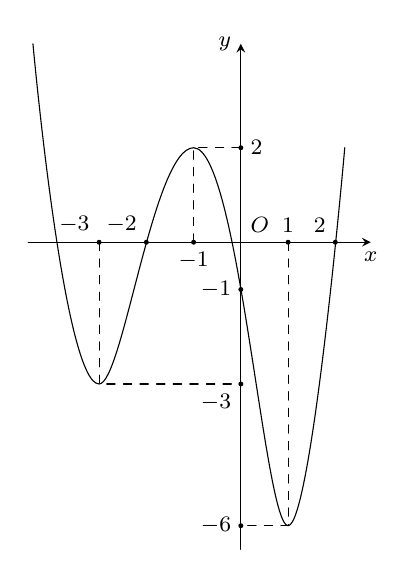
\begin{tikzpicture}[scale=.6, font=\footnotesize, line join=round, line cap=round, >=stealth]
	\def\xmin{-4.5} \def\xmax{2.75}
	\def\ymin{-6.5} \def\ymax{4.2}
	\draw[->] (\xmin,0)--(\xmax,0) node [below]{$x$};
	\draw[->] (0,\ymin)--(0,\ymax) node [left]{$y$};
	\node at (0,0) [above right]{$O$};
	\draw[] (-4.4,4.2)..controls +(0:0) and +(180:0.75)..(-3,-3)
	..controls +(0:0.5) and +(180:0.85)..(-1,2)
	..controls +(0:.95) and +(180:0.5)..(1,-6)
	..controls +(0:0.5) and +(180:0)..(2.2,2);
	\draw[dashed] (-3,0)--(-3,-3)--(0,-3) (-1,0)--(-1,2)--(0,2) (1,0)--(1,-6)--(0,-6);
	\coordinate[label=above left:{$-3$}] (-3x) at (-3,0);
	\coordinate[label=above left:{$-2$}] (-2x) at (-2,0);
	\coordinate[label=below:{$-1$}] (-1x) at (-1,0);
	\coordinate[label=above :{$1$}] (1x) at (1,0);
	\coordinate[label=above left:{$2$}] (2x) at (2,0);
	\coordinate[label=right:{$2$}] (2y) at (0,2);
	\coordinate[label=below left:{$-3$}] (-3y) at (0,-3);
	\coordinate[label=left:{$-6$}] (-6y) at (0,-6);
	\coordinate[label=left:{$-1$}] (-1y) at (0,-1);

	\foreach \p in {-3x,-2x,-1x,1x,2x,2y,-1y,-3y,-6y}
		\fill (\p) circle (1.5pt);
	\end{tikzpicture}
	}
	\loigiai{
	\immini{
	Đặt $t=3x$. Với $x\in\left[-\dfrac{2}{3};\dfrac{2}{3}\right]$ thì $t\in[-2;2]$.\\
	Khi đó
	\[f(3x) + 3x^2 -4x +1 = f(t) + \dfrac{1}{3}t^2 -\dfrac{4}{3}t+1=h(t).\]
	Suy ra $\min\limits_{x\in\left[-\tfrac{2}{3};\tfrac{2}{3}\right]} g(x) = \min\limits_{t\in[-2;2]}h(t)$.\\
	Xét $h(t)=f(t) +\dfrac{1}{3}t^2 - \dfrac{4}{3}t +1$, $t\in[-2;2]$.\\
	$h'(t)=f'(t) + \dfrac{2}{3}t -\dfrac{4}{3}$;\quad $h'(t)=0\Leftrightarrow f'(t)=\dfrac{4}{3}-\dfrac{2}{3}t.\quad (*)$\\
	Ta có $(*)$ là phương trình hoành độ giao điểm của đồ thị hàm số $y=f'(t)$ và đường thẳng $(d)\colon y=\dfrac{4}{3}-\dfrac{2}{3}t$.\\
	Vẽ hai đồ thị trên cùng hệ trục tọa độ như hình vẽ ta có
	}
	{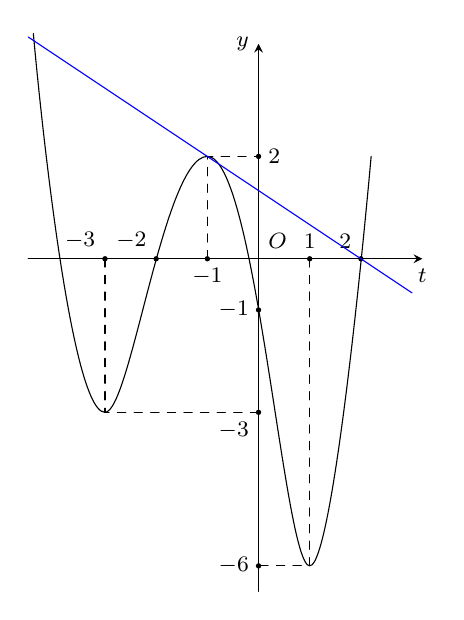
\begin{tikzpicture}[scale=.65, font=\footnotesize, line join=round, line cap=round, >=stealth]
	\def\xmin{-4.5} \def\xmax{3.2}
	\def\ymin{-6.5} \def\ymax{4.2}
	\draw[->] (\xmin,0)--(\xmax,0) node [below]{$t$};
	\draw[->] (0,\ymin)--(0,\ymax) node [left]{$y$};
	\node at (0,0) [above right]{$O$};
	\draw[] (-4.4,4.4)..controls +(0:0) and +(180:0.75)..(-3,-3)
	..controls +(0:0.5) and +(180:0.85)..(-1,2)
	..controls +(0:.95) and +(180:0.5)..(1,-6)
	..controls +(0:0.5) and +(180:0)..(2.2,2);
	\draw[dashed] (-3,0)--(-3,-3)--(0,-3) (-1,0)--(-1,2)--(0,2) (1,0)--(1,-6)--(0,-6);
	\coordinate[label=above left:{$-3$}] (-3x) at (-3,0);
	\coordinate[label=above left:{$-2$}] (-2x) at (-2,0);
	\coordinate[label=below:{$-1$}] (-1x) at (-1,0);
	\coordinate[label=above :{$1$}] (1x) at (1,0);
	\coordinate[label=above left:{$2$}] (2x) at (2,0);
	\coordinate[label=right:{$2$}] (2y) at (0,2);
	\coordinate[label=below left:{$-3$}] (-3y) at (0,-3);
	\coordinate[label=left:{$-6$}] (-6y) at (0,-6);
	\coordinate[label=left:{$-1$}] (-1y) at (0,-1);

	\foreach \p in {-3x,-2x,-1x,1x,2x,2y,-1y,-3y,-6y}
		\fill (\p) circle (1.5pt);
	\draw[blue,smooth,samples=200,domain=-4.5:3] plot (\x,{-2/3*(\x)+4/3});
	\end{tikzpicture}}
	\[f'(t)=\dfrac{4}{3}-\dfrac{2}{3}t \Leftrightarrow \hoac{&t=a \quad(a<-3)\\&t=-1 \quad (\text{nghiệm bội chẵn})\\& t=2}\]
	Bảng biến thiên của $y=h(t)$ trên $[-2;2]$
	\begin{center}
	
\begin{tikzpicture}
	\tkzTabInit[nocadre,lgt=1.5,espcl=2.5,deltacl=0.85]
	{$t$/0.6,$h'(t)$/0.6,$h(t)$/2}{$-2$,$-1$,$2$}
	\tkzTabLine{,-,0,-,0}
	\tkzTabVar{+/$h\left(-2\right)$,R,-/$h\left(2\right)$}
	\end{tikzpicture}
	\end{center}
	Từ bảng biến thiên ta có $\min\limits_{x\in\left[-\tfrac{2}{3};\tfrac{2}{3}\right]} g(x) = \min\limits_{t\in[-2;2]}h(t)=h(2)=f(2)-\dfrac{1}{3}$.
}
\end{ex}

%Câu 46
\begin{ex}%[Dự án 16 - TeamTeXHoa - TT Kim Liên-HN-L1 - Nguyễn Thắng]%[2D3G1-2]
	Cho hàm số $f\left( x \right)$ thỏa mãn $f\left( x \right)>0,\forall x>\dfrac{1}{2}$ và có đạo hàm $f'\left( x \right)$ liên tục trên khoảng $\left( \dfrac{1}{2};+\infty \right)$ thỏa mãn $f'\left( x \right)+8xf^2\left( x \right)=0,\forall x>\dfrac{1}{2}$ và $f\left( 1 \right)=\dfrac{1}{3}$. Tính $f\left( 1 \right)+f\left( 2 \right)+\cdots +f\left( 1011 \right)$.
	\choice
	{\True $\dfrac{1}{2}\cdot\dfrac{2022}{2023}$}
	{$\dfrac{2021}{2043}$}
	{$\dfrac{2022}{4045}$}
	{$\dfrac{1}{2}\cdot\dfrac{2021}{2022}$}
	\loigiai{
	Với mọi $x>\dfrac{1}{2}$, ta có
	$$f'\left( x \right)+8xf^2\left( x \right)=0\Leftrightarrow \dfrac{-f'\left( x \right)}{f^2\left( x \right)}=8x\Leftrightarrow \displaystyle\int{\dfrac{-f'\left( x \right)}{f^2\left( x \right)}\mathrm{\,d}x}=\displaystyle\int{8x}\mathrm{\,d}x\Leftrightarrow \dfrac{1}{f\left( x \right)}=4x^2+C.$$
	Mà $f\left( 1 \right)=\dfrac{1}{3}\Rightarrow C=-1$.\\
	Vậy $f\left( x \right)=\dfrac{1}{4x^2-1}=\dfrac{1}{2}\left( \dfrac{1}{2x-1}-\dfrac{1}{2x+1} \right),\,\forall x >\dfrac{1}{2}$.\\
	Ta có\\
	$\left. \begin{aligned}
	& f\left( 1 \right)=\dfrac{1}{2}\left( 1-\dfrac{1}{3} \right) \\
	& f\left( 2 \right)=\dfrac{1}{2}\left( \dfrac{1}{3}-\dfrac{1}{5} \right) \\
	&.... \\
	& f\left( 1011 \right)=\dfrac{1}{2}\left( \dfrac{1}{2021}-\dfrac{1}{2023} \right) \\
	\end{aligned} \right\}\Rightarrow T=f\left( 1 \right)+f\left( 2 \right)+\cdots+f\left( 1011 \right)=\dfrac{1}{2}\left( 1-\dfrac{1}{2023} \right)=\dfrac{1}{2}\cdot\dfrac{2022}{2023}$.}
\end{ex}

%Câu 47
\begin{ex}%[Dự án 16 - TeamTeXHoa - TT Kim Liên-HN-L1 - Nguyễn Thắng]%[2D2K6-5]
	Cho bất phương trình $\log_5\left( x^2-4x+4+m \right)-1<\log_5\left( x^2+2x+3 \right)$ với $m$ là tham số. Có tất cả bao nhiêu giá trị nguyên của tham số $m$ để bất phương trình nghiệm đúng với mọi $x$ thuộc khoảng $\left( 1;3 \right)$?
	\choice
	{$30$}
	{$28$}
	{\True $29$}
	{Vô số}
	\loigiai{
	Ta có
	\begin{eqnarray*}
		\log_5\left( x^2-4x+4+m \right)-1<\log_5\left( x^2+2x+3 \right)
		&\Leftrightarrow&{\log_5}\left( x^2-4x+4+m \right)<\log_5\left( 5x^2+10x+15 \right)\\
		&\Leftrightarrow&\heva{&5x^2+10x+15>x^2-4x+4+m \\&x^2-4x+4+m>0}\\
		&\Leftrightarrow&\heva{&4x^2+14x+11>m \quad\left( 1 \right) \\&x^2-4x+4>-m.\quad\left( 2 \right)}
	\end{eqnarray*}	
	\begin{itemize}
		\item Xét $f\left( x \right)=4x^2+14x+11$ trên $\left( 1;3 \right)$.\\
		Ta có $f'\left( x \right)=8x+14>0,\, \forall x\in \left( 1;3 \right)$.\\
		Suy ra $(1)$ nghiệm đúng $\forall x \in (1;3)$ khi $m\le f\left( 1 \right)=29$.
		\item Xét $g\left( x \right)=x^2-4x+4$ trên $\left( 1;3 \right)$.\\
		Ta có bảng biến thiên của $g\left( x \right)$ trên $\left( 1;3 \right)$
	\begin{center}
	
\begin{tikzpicture}
	\tkzTabInit[nocadre,lgt=1.2,espcl=2.5,deltacl=0.6]
	{$x$/0.6,$g(x)$/2}{$1$,$2$,$3$}
	\tkzTabVar{+/$1$,-/$0$,+/$4$}
	\end{tikzpicture}
	\end{center}
	Suy ra $(2)$ nghiệm đúng $\forall x\in (1;3)$ khi $-m< 0\Leftrightarrow m> 0$.
	\end{itemize}
	Từ các kết quả trên ta có bất phương trình ban đầu nghiệm đúng với mọi $x\in (1;3)$ khi $0< m\le 29$.\\
	Vậy có $29$ giá trị nguyên của tham số $m$.}
\end{ex}

%Câu 48
\begin{ex}%[Dự án 16 - TeamTeXHoa - TT Kim Liên-HN-L1 - Nguyễn Thắng]%[2D2G5-5]
	Gọi $S$ là tập nghiệm của phương trình $\left(2^x+3^x-8x+3 \right)\sqrt{\left( 3 \right)^{2^x}-m}=0$ (với $m$ là tham số thực). Có tất cả bao nhiêu giá trị nguyên của $m\in \left[-2021;2021 \right]$ để tập hợp $S$ có đúng hai phần tử?
	\choice
	{\True $2095$}
	{$2092$}
	{$2093$}
	{$2094$}
	\loigiai{
	Điều kiện: $\left( 3 \right)^{2^x}-m\ge 0$.\\
	Ta có\\
	$$\left(2^x+3^x-8x+3 \right)\sqrt{\left( 3 \right)^{2^x}-m}=0\Leftrightarrow \hoac{&2^x+3^x-8x+3=0\quad(1) \\&\left( 3 \right)^{2^x}=m.\quad (2)}$$
	\begin{itemize}
		\item Giải $(1)$:\\
		Xét hàm số $f\left( x \right)=2^x+3^x-8x+3$.\\
		Ta có $f'\left( x \right)=2^x\ln 2+3^x\ln 3-8$.\\
		Nhận xét rằng $f(x)$, $f'(x)$ là các hàm liên tục trên $\mathbb{R}$.\\
		Vì $f''\left( x \right)=2^x\left( \ln 2 \right)^2+3^x\left( \ln 3 \right)^2>0,\forall x\in \mathbb{R}$ nên phương trình $f'\left( x \right)=0$ có nhiều nhất là $1$ nghiệm. Suy ra phương trình $f(x)=0$ có nhiều nhất $2$ nghiệm.\\
		Mặt khác, $x=1$ và $x=2$ là hai nghiệm của phương trình. Vậy $S_1=\{1;2\}$.
		\item Giải $(2)$:\\
		+ Với $m\leq 1$, ta có $S_2=\varnothing$.\\
		+ Với $m>1$, ta có $S_2=\{\log_2\left(\log_3 m\right)\}$.
	\end{itemize}
	Từ điều kiện xác định, nhận xét rằng nếu $x=1$ là thỏa mãn thì $x=2$ cũng thỏa mãn.\\
	Để phương trình ban đầu có đúng $2$ nghiệm, ta có các trường hợp sau:
	\begin{itemize}
		\item {\bf Trường hợp 1:} Phương trình ban đầu có $S=\{1;2\}$.\\ 
		Khi đó $x=1$ thỏa mãn điều kiện và phương trình $(2)$ vô nghiệm hoặc có nghiệm trùng với nghiệm của phương trình $(1)$.
		\[\heva{&3^{2^1}-m\geq 0\\&\hoac{&m\leq 1\\&\log_2(\log_3 m)=1\\&\log_2\left(\log_3 m\right)=2}}\Leftrightarrow\heva{&m\leq 9\\&\hoac{&m\leq 1\\&m=9\\& m=81}}\Leftrightarrow \hoac{&m=9\\&m\leq 1.}\]
		\item {\bf Trường hợp 2:} Phương trình ban đầu có $S=\{2;\log_2\left(\log_3(m)\right)\}$.\\
		Khi đó $x=1$ không thỏa mãn điều kiện, $x=2$ thỏa mãn điều kiện và phương trình $(2)$ có nghiệm khác $2$.
		\[\heva{&3^{2^{1}}-m<0\\&3^{2^{2}}-m\geq 0\\&m>1\\&\log_2\left(\log_3 m\right)\neq 2} \Leftrightarrow \heva{&m>9\\& m\leq 81\\&m>1\\&m\neq 81}\Leftrightarrow 9<m<81.\]
	\end{itemize}
	Từ hai trường hợp, ta được $\hoac{&m\leq 1\\&9\leq m<81.}$\\
	Mà $m$ nhận giá trị nguyên và $m\in[-2021;2021]$ nên $m\in\{-2021;\ldots;1;9;10;\ldots;80\}$.\\
	Vậy có $2095$ giá trị $m$ thỏa yêu cầu.
	}
\end{ex}

%Câu 49
\begin{ex}%[Dự án 16 - TeamTeXHoa - TT Kim Liên-HN-L1 - Nguyễn Thắng]%[2H3G2-8]
	Trong không gian $Oxyz$, cho hai điểm $A\left( -1;2;3 \right)$ và $B\left( 3;2;5 \right)$. Xét hai điểm $M$ và $N$ thay đổi thuộc mặt phẳng $\left( Oxy \right)$ sao cho $MN=2023$. Tìm giá trị nhỏ nhất của $AM+BN$.
	\choice
	{$2\sqrt{17}$}
	{$\sqrt{65}$}
	{$25\sqrt{97}$}
	{\True $205\sqrt{97}$}
	\loigiai{
	\begin{center}
	\begin{tikzpicture}[scale=.85, font=\footnotesize, line join=round, line cap=round, >=stealth]
	\path (4,2)coordinate[label=left:$A$](A) (4,-2)coordinate[label=below:$A'$](A') (8,5)coordinate[label=above:$B$](B) (10,5)coordinate[label=above right:$B'$](B') (7,0)coordinate[label=below:$N$](N) (9,0)coordinate[label=below:$M$](M) (4,4.5)coordinate[label=left:$H$](H) (0,-1)coordinate[label=center:](E) (1,1)coordinate[label=center:](F) (11,1)coordinate[label=center:](I) (10,-1)coordinate[label=center:](J) (0,4)coordinate[label=center:](O) (1,6)coordinate[label=center:](K) (12,6)coordinate[label=center:](P) (11,4)coordinate[label=center:](Q)
	(6.5,-1)coordinate[label=center:](R) (4,0)coordinate[label=center:](H') (4,4)coordinate[label=center:](S)(4,-1)coordinate[label=center:](S');
	\draw pic[draw,blue,angle radius=10mm] {angle = J--E--F};8
	\draw (0.6,-0.7)node[]{$Oxy$};
	\draw pic[draw,blue,angle radius=8mm] {angle = Q--O--K};
	\draw (0.46,4.34)node[]{$P$};
	\draw (E)--(F)--(I)--(J)--(E) (O)--(K)--(P)--(Q)--(O) (H')--(A)--(M) (H)--(B') (A')--(R) (A)--(S) (A')--(S'); 
	\draw[blue] (N)--(B) (M)--(B'); 
	\draw (N)--(M) (B)--(B');
	\draw[dashed] (M)--(R) (H)--(S) (H')--(S');
	\foreach \diem in {A,A',B,B',N,M,H} \fill (\diem)circle(1.5pt);
	\draw[red,dashed] (B) ellipse (2cm and 0.75cm);
	\end{tikzpicture}
	\end{center}
	\begin{itemize}
		\item {\bf Lập luận giá trị nhỏ nhất}:\\
		- Nhận xét rằng  $z_A>0$, $z_B>0$ nên hai điểm $A$, $B$ nằm cùng phía so với $
		(Oxy)$.
		\begin{itemize}
			\item[+] Dựng $A'$ đối xứng với $A$ qua $\left( Oxy \right)$. Suy ra $AM=A'M$.
			\item[+] Dựng $\overrightarrow{B'M}=\overrightarrow{BN}$. Suy ra $BN=B'M$.
		\end{itemize}
		Từ đó ta có $AM + BN = A'M + B'M \geq A'B'$.\\
		- Nhận xét rằng $A'$ cố định và $B'$ di động. Ta sẽ tìm vị trí của $B'$ để $A'B'$ đạt giá trị nhỏ nhất.\\
		- Vì $B$ cố định, $BB'\parallel (Oxy)$ và $BB'=MN=2023$ nên $B'$ di động trên đường tròn $(C)$ tâm $B$, bán kính $R=2023$ và nằm trong mặt phẳng $(P)\parallel (Oxy)$.\\
		Gọi $H$ là hình chiếu của $A'$ lên $(P)$. Ta có $A'$, $H$, $B$ cố định nên $A'H$, $HB$ không đổi.\\
		Khi đó
		\[A'B'=\sqrt{A'H^2 + HB'^2} \Rightarrow A'B'_{\min}\Leftrightarrow HB'_{\min}=|HB - BB'|.\]
		\item {\bf Tính giá trị nhỏ nhất}:\\
		Điểm $A'$ đối xứng với $A(-1;2;3)$ qua $(Oxy)$ nên $A'(-1;2;-3)$.\\
		Mặt phẳng $(P)$ qua $B(3;2;5)$ và song song $(Oxy)\colon z=0$ nên $(P)\colon z=5$.\\
		Điểm $H$ là hình chiếu của $A'(-1;2;-3)$ lên $(P)\colon z=5$, ta tìm được $H(-1;2;5)$.\\
		Ta có $\overrightarrow{HB}=(4;0;0)$; $\overrightarrow{A'H}=(0;0;8)\Rightarrow HB=4$; $A'H=8$.\\
		Khi đó $HB'\geq |HB-BB'|=|4-2023|=2019$.
		Suy ra
		 \[AM +BN \geq A'B' =\sqrt{A'H^2 + HB'^2}\geq \sqrt{8^2 +2019^2}=205\sqrt{97}.\]
	\end{itemize}
	Vậy giá trị nhỏ nhất cần tìm là $205\sqrt{97}$.
	}
\end{ex}

%Câu 50
\begin{ex}%[Dự án 16 - TeamTeXHoa - TT Kim Liên-HN-L1 - Nguyễn Thắng]%[2D1G2-6]
	Cho hàm số $f\left( x \right)$ có đạo hàm trên $\mathbb{R}$ là $f'\left( x \right)=\left( x+3 \right)\left( x-4 \right)$. Tính tổng các giá trị nguyên của tham số $m\in \left[-10;5 \right]$ để hàm số $y=f\left( \left| x^2-3x+m \right| \right)$ có nhiều điểm cực trị nhất.
	\choice
	{$54$}
	{$9$}
	{$-52$}
	{\True $-54$}
	\loigiai{
	Ta có $f'\left( x \right)=\left( x+3 \right)\left( x-4 \right)=0\Leftrightarrow \hoac{&x=-3 \\&x=4.}$\\
	Tính đạo hàm, $y'=f'\left( \left| x^2-3x+m \right| \right)\dfrac{x^2-3x+m}{\left| x^2-3x+m \right|}\left( 2x-3 \right)$.\\
	$y'=0\Leftrightarrow \hoac{&x=\dfrac{3}{2} \\&x^2-3x+m=0 \\&\left| x^2-3x+m \right|=-3\left(\text{vô nghiệm}\right) \\&\left| x^2-3x+m \right|=4}\Leftrightarrow \hoac{&x=\dfrac{3}{2} \\&x^2-3x+m=0 \\&x^2-3x+m=4 \\&x^2-3x+m=-4}\Leftrightarrow \hoac{&x=\dfrac{3}{2} \\&x^2-3x=-m\\&x^2-3x=4-m\\&x^2-3x=-4-m.}$\\
	Đặt $g\left( x \right)=x^2-3x$, khảo sát hàm số $y=g\left( x \right)$, ta được bảng biến thiên như bên dưới.
	\begin{center}
	\begin{tikzpicture}
	\tkzTabInit[nocadre,lgt=1.2,espcl=3,deltacl=0.6]
	{$x$/1.1,$g(x)$/4}{$-\infty$,$\dfrac{3}{2}$,$+\infty$}
	%	\tkzTabLine{,-,0,+,}
	\tkzTabVar{+/$+\infty$,-/$-\dfrac{9}{4}$,+/$+\infty$}
	\draw[red] (2,-3.5)--(7,-3.5);\draw (7,-3.5)node[right]{$y=-m-4$};
	\draw[red] (2,-3)--(7,-3);\draw (7,-3)node[right]{$y=-m$};
	\draw[red] (2,-2.5)--(7,-2.5);\draw (7,-2.5)node[right]{$y=-m+4$};
	\end{tikzpicture}
	\end{center}
	Hàm số có nhiều điểm cực trị nhất khi và chỉ khi $-m-4>\dfrac{-9}{4}\Leftrightarrow m<-\dfrac{7}{4}$.\\
	Kết hợp với điều kiện $m\in \mathbb{Z}$, $m\in \left[-10;5 \right]$ suy ra tập giá trị $m$ là $\left\{-10;-9;-8;\ldots;-2 \right\}$.\\
	Vậy tổng các giá trị nguyên của tham số $m$ bằng $-54$.}
\end{ex}

\Closesolutionfile{ans}